\section{The Diffraction Grating}

\makelabheader

\answerspace{1in}

All sorts of waves, including light, do a couple 
of strange things:
\begin{enumerate}
\item Waves bend (a bit) around corners, and spread
out (a bit) when passing through holes. 
This phenomenon is called {\it diffraction}.
\item When two waves meet each other, they
can cancel each other out (if ``peaks'' of the
first wave run into ``valleys'' from the second), 
or they can reinforce each other (if peaks meet up with peaks).
This is called {\it interference}.
\end{enumerate}

A diffraction grating is a device
that takes advantage of both of these phenomena.  They turn
out to be very useful in measuring the wavelength
of light and in splitting light up into its constituent
wavelengths.  

A diffraction grating is just a piece of glass (or something similar)
with many thin parallel lines ruled on it.  When light passes through
the small gaps between these lines, it diffracts.  Light that passed
through the various gaps can then interfere with each other.  In some
directions, the waves that passed through the various gaps cancel each
other out, and in other directions they reinforce each other.  The
result is a pattern of alternating bright and dark patches.

Suppose we take light with wavelength $\lambda$ and
shine it through a diffraction grating.  We then
project the light on a wall and measure the 
positions $x$ of the bright spots (relative to the
center of the diffraction pattern) as shown.  The theory of 
interference tells us that 
\begin{displaymath} n\lambda = {dx\over \sqrt{L^2+x^2}}.  \end{displaymath}
Here $d$ is the separation between lines in the grating and $L$
is the distance from the grating to the wall.  $n$ is called the
``order'' of the spot; it's just an integer: $n=1,2,3,\ldots$.

Note that there are four different quantities in this expression that
have units of length.  One common source of error is to
use incompatible units for these things.  The safest thing is
to use the same units for all four.

One nice thing we can do with all this is measure the wavelength of light.

\bigskip
%\centerline{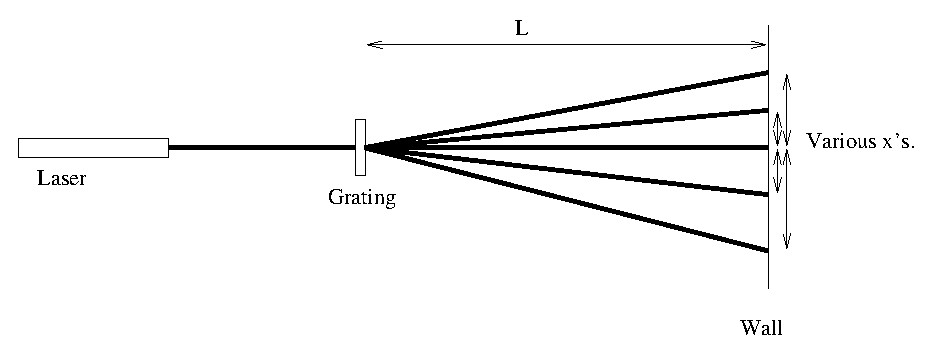
\includegraphics{figs/difffig.eps}}
\bigskip

\begin{enumerate}
\item Record the separation between grating lines: \( d= \)
\item Turn on the laser, being careful to avoid looking directly into the
beam or shining it at anyone. Aim the light beam through the diffraction
grating so that a horizontal series of dots appears on the wall. Adjust
the positions of the laser and grating until you easily see at least
two dots on either side of the brightest (central) dot.
\item Are the dots of the interference/diffraction pattern the same intensity?
Describe the pattern you observe.\answerspace{15mm}

\item Measure the distance from the grating to the wall, $L$,
as well as the distances from the central dot to the first dot to
the right, $x$, and the first dot to the left, $x'$. Compute the average
of these $x$ values and record it as $x_{ave}$. Record all of these
values in the table below.
\item Use the equation above to find the wavelength $\lambda$.
Because these are the first two spots (other than the central dot),
use the value $n=1$.
\item Repeat the procedure using the second dot to the right
of center and the second dot to the left.  This time, use $n=2$ 
when finding the wavelength.
\item If you can see the third pair of dots clearly, repeat the
procedure with $n=3$.
\item Move the laser to a new location (that is, change the
value of $L$) and repeat the procedure for a couple of values
of $n$.  In the end, you should end up with at least
five different determinations of $\lambda$.
\item Compute the average of your determinations of the laser light's
  wavelength and compare it to the expected value, which is printed on the
  laser.
\answerspace{15mm}

\end{enumerate}
\answerspace{0.3cm}
\begin{center}
\begin{tabular}{|c|c|c|c|c|}
\hline 
\( L \) (cm)&
\( x \) (cm)&
\( x' \) (cm)&
\( x_{ave} \) (cm)&
\( \lambda  \) (nm)\\
\hline
\hline 
&
&
&
&
\\
&
&
&
&
\\
\hline 
&
&
&
&
\\
&
&
&
&
\\
\hline 
&
&
&
&
\\
&
&
&
&
\\
\hline 
&
&
&
&
\\
&
&
&
&
\\
\hline 
&
&
&
&
\\
&
&
&
&
\\
\hline
\end{tabular}\answerspace{0.3cm}

\end{center}


Suppose that we shone white light instead of laser light
through the grating.  What would the resulting pattern look
like?
